\documentclass[11pt]{article}
\usepackage[margin=1in]{geometry}
\usepackage{graphicx}
\usepackage{booktabs}
\usepackage{amsmath}
\usepackage{hyperref}
\usepackage{xcolor}

\title{W125--W134 Calibration Report:\\Per-Site Flushing Worsens RMSE---and Why}
\author{Anton Star (automated analysis)}
\date{March 8, 2026}

\begin{document}
\maketitle

\section{Executive Summary}

Per-site flushing derived from enclosedness metrics \textbf{worsened calibration fit} across all configurations tested. The best run (W129, $\alpha_\text{env}=0.25$) achieved RMSE=0.691, compared to W117's 0.603 under uniform $\phi=0.5$. This report argues this is not a bug---it reveals a \textbf{fundamental asymmetry in how flushing affects disease dynamics}, and points toward the missing mechanism (salinity).

\section{The Argument}

\subsection{What Per-Site Flushing Changed}

Under uniform $\phi=0.5$, all 896 sites flushed pathogen at the same rate. The north-south recovery gradient was driven entirely by SST-modulated $\alpha_\text{env}$ (warm south $\rightarrow$ more disease amplification).

Per-site flushing introduced two changes simultaneously:
\begin{enumerate}
    \item \textbf{Enclosed sites (AK fjords, Salish Sea)}: $\phi$ dropped from 0.50 $\rightarrow$ 0.28--0.30
    \item \textbf{Open coast (CA, OR)}: $\phi$ rose from 0.50 $\rightarrow$ 0.66--0.68
\end{enumerate}

\subsection{Why This Made Things Worse}

The $P_\text{env}$ dynamics at each node follow:
\begin{equation}
\frac{dP}{dt} = \underbrace{\text{shedding}}_{\text{infected hosts}} - \underbrace{\xi \cdot P}_{\text{decay}} - \underbrace{\phi \cdot P}_{\textbf{flushing}} + \underbrace{\text{dispersal}}_{\text{D matrix}} + \underbrace{\text{floor}}_{\alpha_\text{env}}
\end{equation}

Lower $\phi$ means pathogen decays more slowly locally. For enclosed AK fjord sites:
\begin{itemize}
    \item $\phi$ dropped from 0.5 to $\sim$0.3 $\rightarrow$ local $P_\text{env}$ accumulates 67\% more
    \item Disease pressure \textit{increases} $\rightarrow$ populations recover \textit{less}
    \item AK-PWS recovery: 7.85\% (W117) $\rightarrow$ 3.74\% (W129)---\textbf{moving away from the 50\% target}
\end{itemize}

For open coast CA/OR sites:
\begin{itemize}
    \item $\phi$ rose from 0.5 to $\sim$0.67 $\rightarrow$ pathogen flushes 34\% faster
    \item Disease pressure \textit{decreases} $\rightarrow$ populations recover \textit{more}
    \item CA-N recovery: 0.19\% (W117) $\rightarrow$ 0.43\% (W129)---\textbf{moving away from the 0.1\% target}
\end{itemize}

\textbf{Both effects push RMSE upward}. Per-site flushing counteracts the SST-driven gradient: it makes the north sicker (where we need recovery) and the south healthier (where we need suppression).

\subsection{The D Matrix Partially Compensates}

The pathogen dispersal matrix is modulated by source $\phi$:
$$D[j,k] = \phi_j \cdot f_\text{out} \cdot \exp(-d_{jk}/D_P) \cdot S_{jk}$$

So enclosed sites (low $\phi_j$) export less pathogen. This \textit{should} protect enclosed neighbors. But the effect is asymmetric:
\begin{itemize}
    \item \textbf{Export reduction}: enclosed sites shed less to neighbors (helpful)
    \item \textbf{Local retention}: enclosed sites retain own $P_\text{env}$ longer (\textbf{harmful, and dominant})
    \item \textbf{Import unchanged}: incoming pathogen from the wavefront isn't modulated by recipient $\phi$
\end{itemize}

Once disease arrives via the wavefront (which uses its own long-range kernel), local retention dominates. The wavefront D matrix is independent of $\phi$---so the initial disease import is identical, but the local response differs dramatically.

\subsection{The Real World is Different}

Empirically, enclosed waterways like Prince William Sound \textit{are} refuges (Gehman et al. 2025, Proc Royal Soc B). But the protection mechanism isn't flushing dynamics---it's:

\begin{enumerate}
    \item \textbf{Salinity}: Freshwater lens in fjords (glacial melt, river input) directly kills \textit{Vibrio} (halophilic; need $>$0.5\% NaCl). PWS surface salinity drops to 20 PSU seasonally.
    \item \textbf{Depth refuge}: Low salinity at surface pushes \textit{Pycnopodia} deeper into cold water, below the \textit{Vibrio} activity threshold.
\end{enumerate}

Our model captures temperature (SST) but \textbf{not salinity}. Without salinity, per-site flushing can only encode one relationship: enclosed $\rightarrow$ retains pathogen $\rightarrow$ more disease. This is physically correct but biologically incomplete. The real protective mechanism (salinity killing \textit{Vibrio}) is absent.

\section{Results}

\subsection{RMSE Comparison}

\begin{figure}[h]
\centering
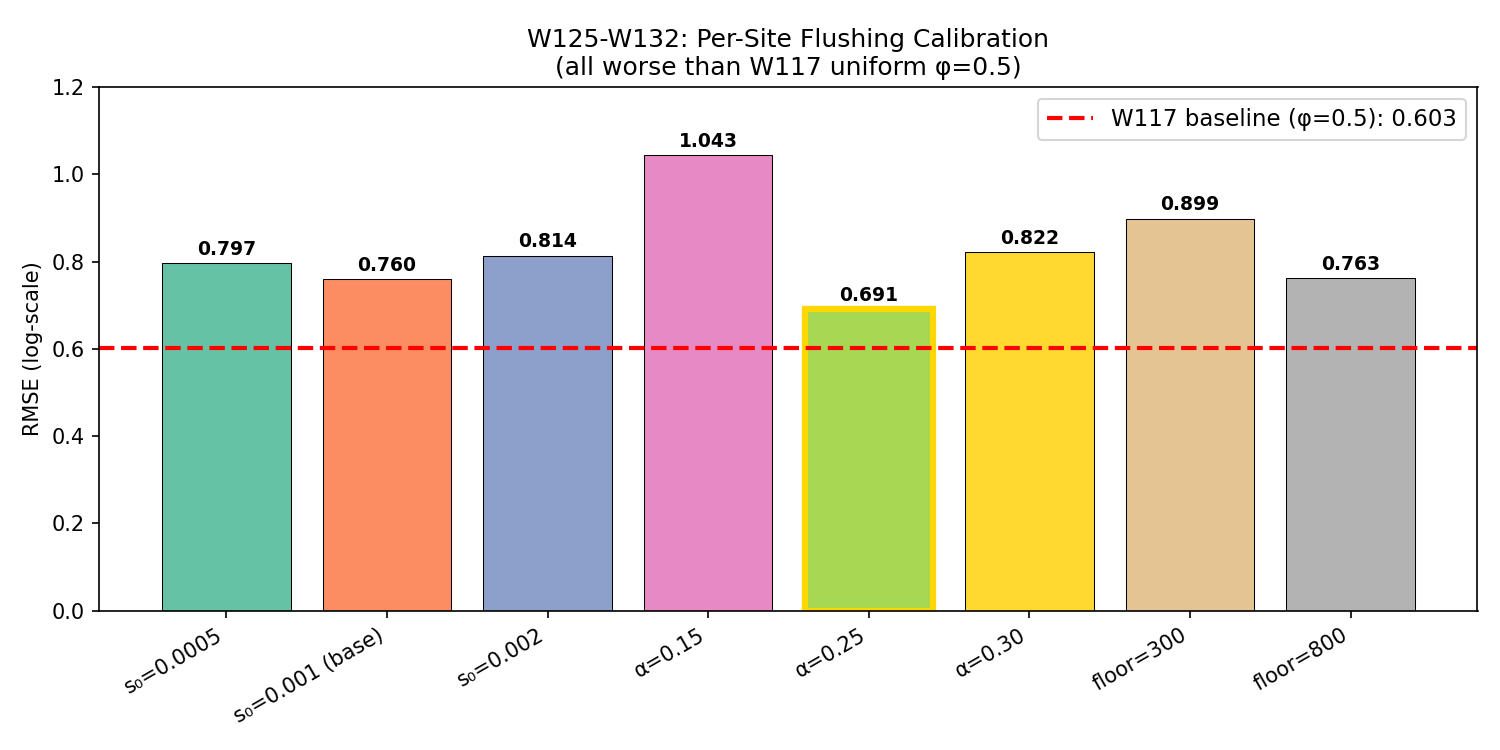
\includegraphics[width=\textwidth]{figures/fig1_rmse_comparison.png}
\caption{All W125--W132 runs score worse than the W117 baseline (uniform $\phi=0.5$, dashed red line). W129 ($\alpha=0.25$) is the best at 0.691 but still 15\% worse than W117 (0.603).}
\end{figure}

\subsection{Regional Breakdown}

\begin{figure}[h]
\centering
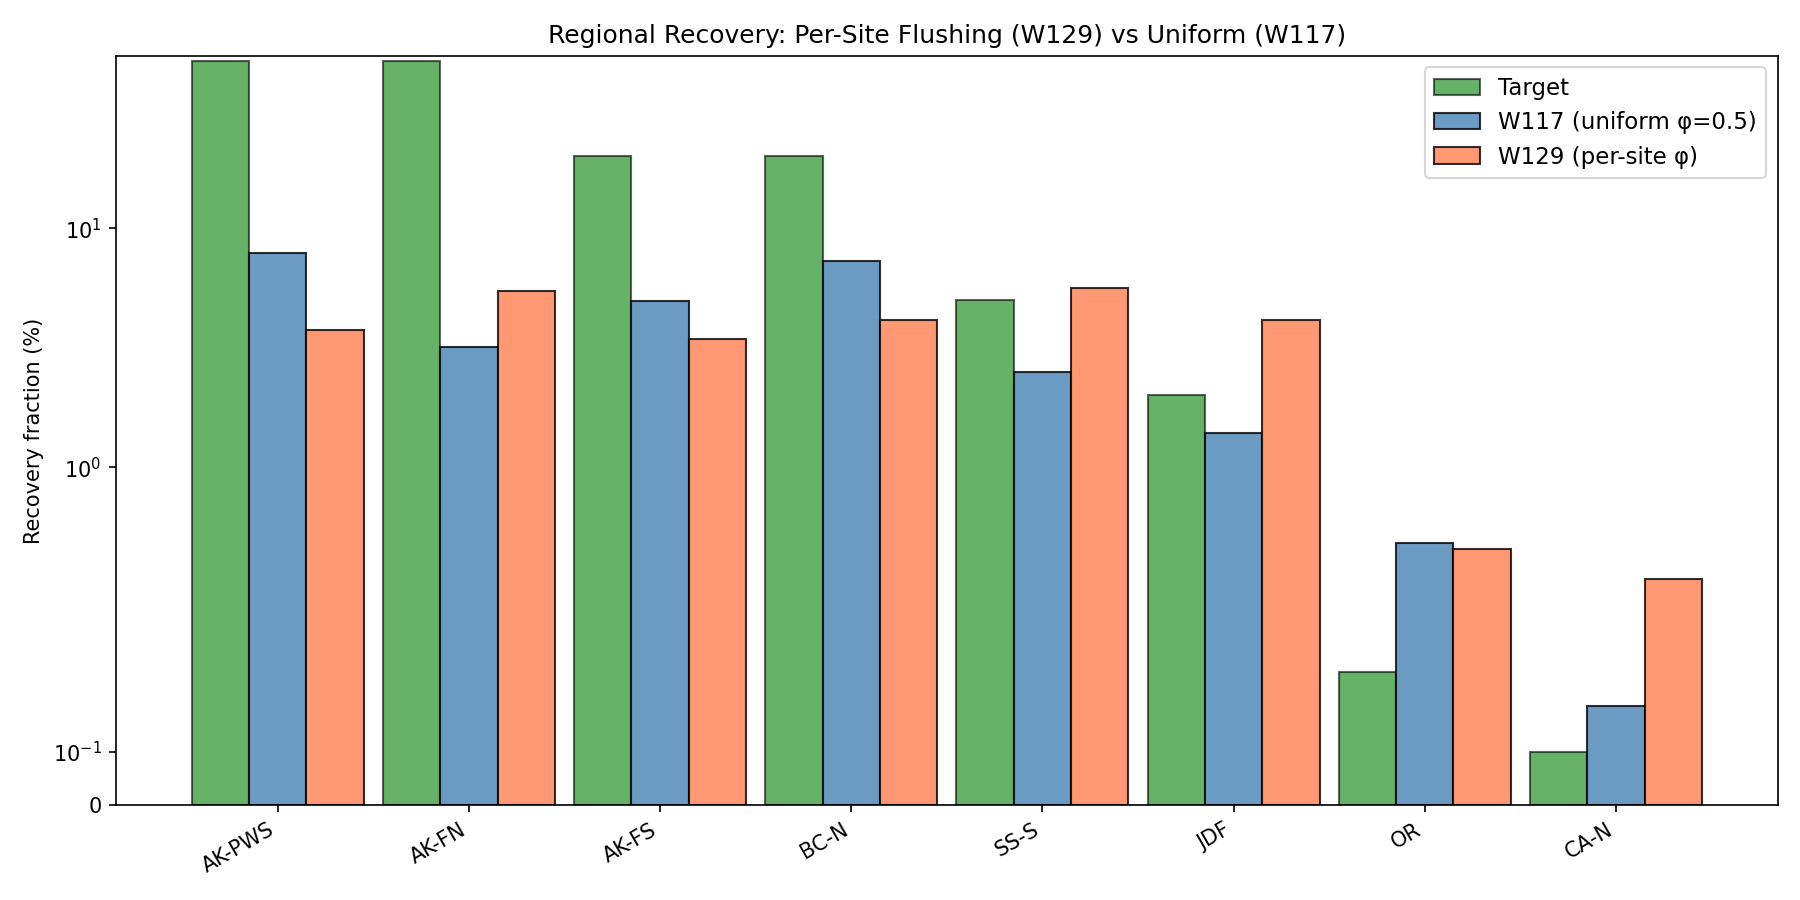
\includegraphics[width=\textwidth]{figures/fig2_regional_comparison.png}
\caption{Per-region recovery comparison. W117 (blue) nails the south (SS-S, JDF, OR, CA-N all close to targets). W129 (orange) overshoots the south while undershoting the north---the gradient is flatter.}
\end{figure}

\begin{figure}[h]
\centering
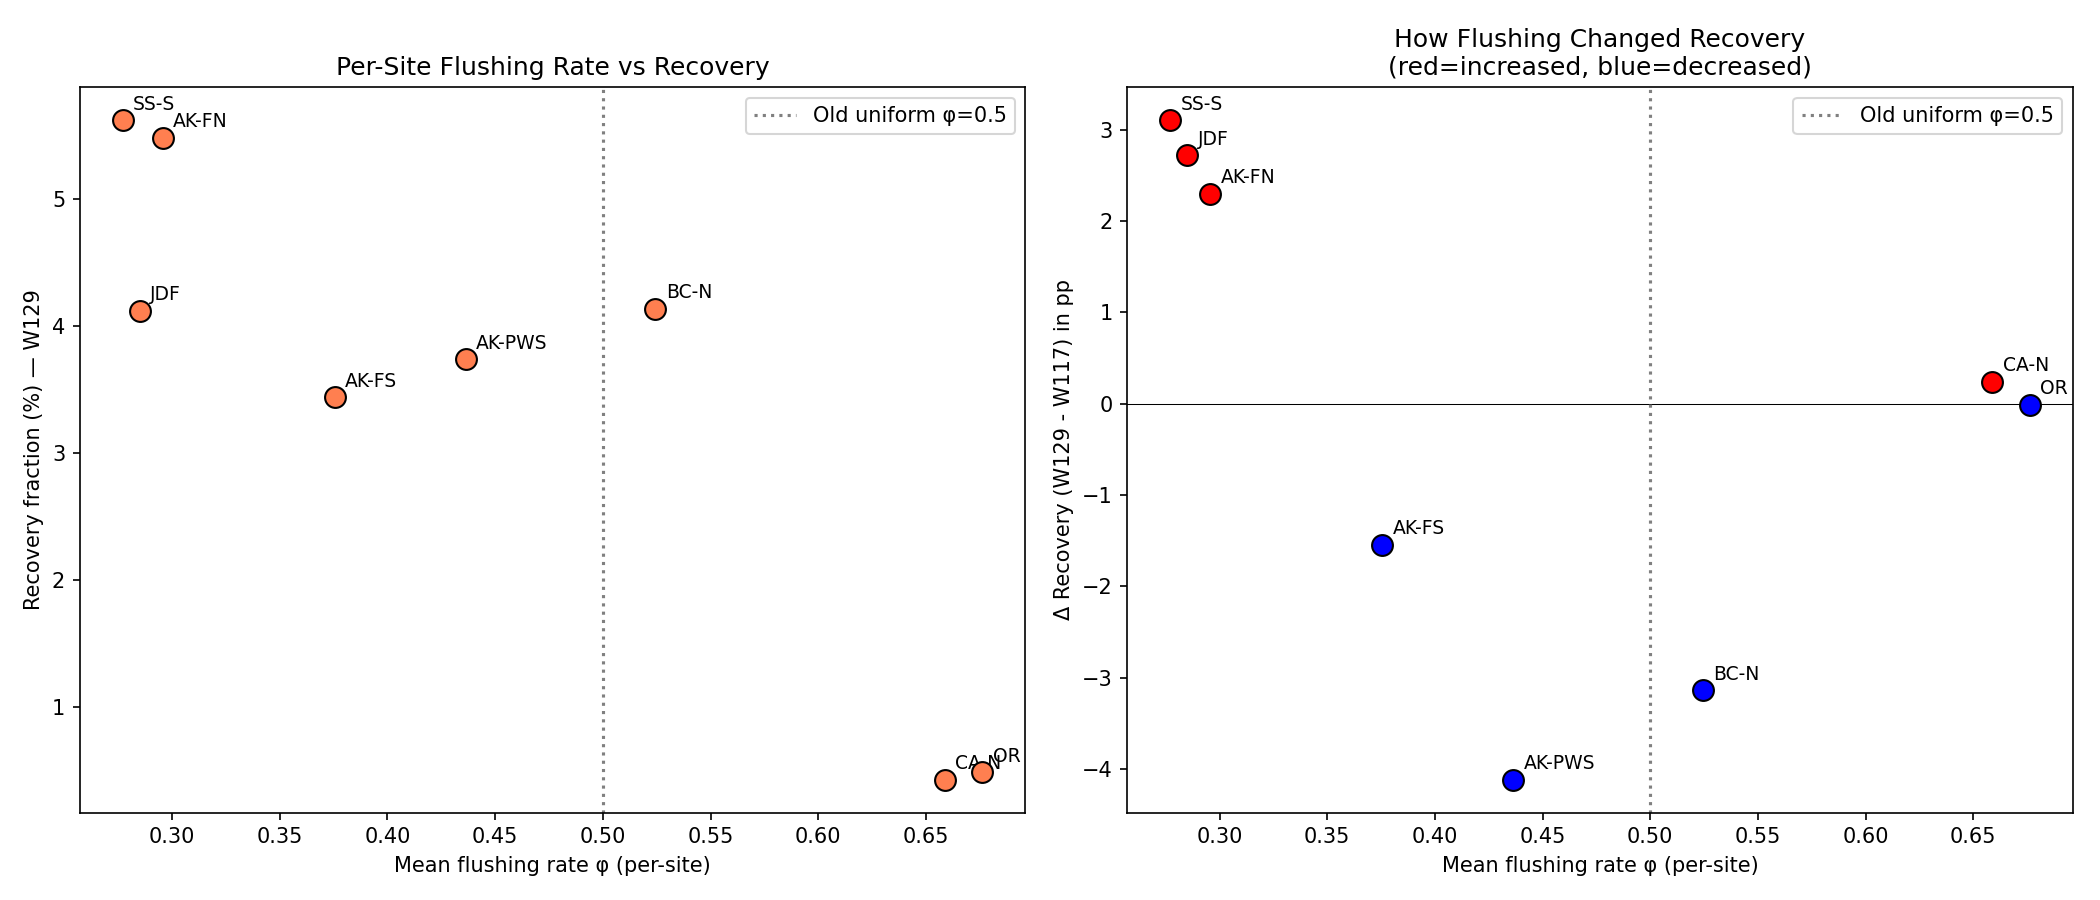
\includegraphics[width=\textwidth]{figures/fig3_flushing_mechanism.png}
\caption{\textbf{Left}: Mean regional $\phi$ vs recovery. Low-$\phi$ regions (enclosed) have low recovery. \textbf{Right}: Change from W117. Regions that got lower $\phi$ (below old 0.5) lost recovery; regions that got higher $\phi$ gained recovery. The flushing change systematically pushes the gradient in the wrong direction.}
\end{figure}

\subsection{Recovery Trajectories}

\begin{figure}[h]
\centering
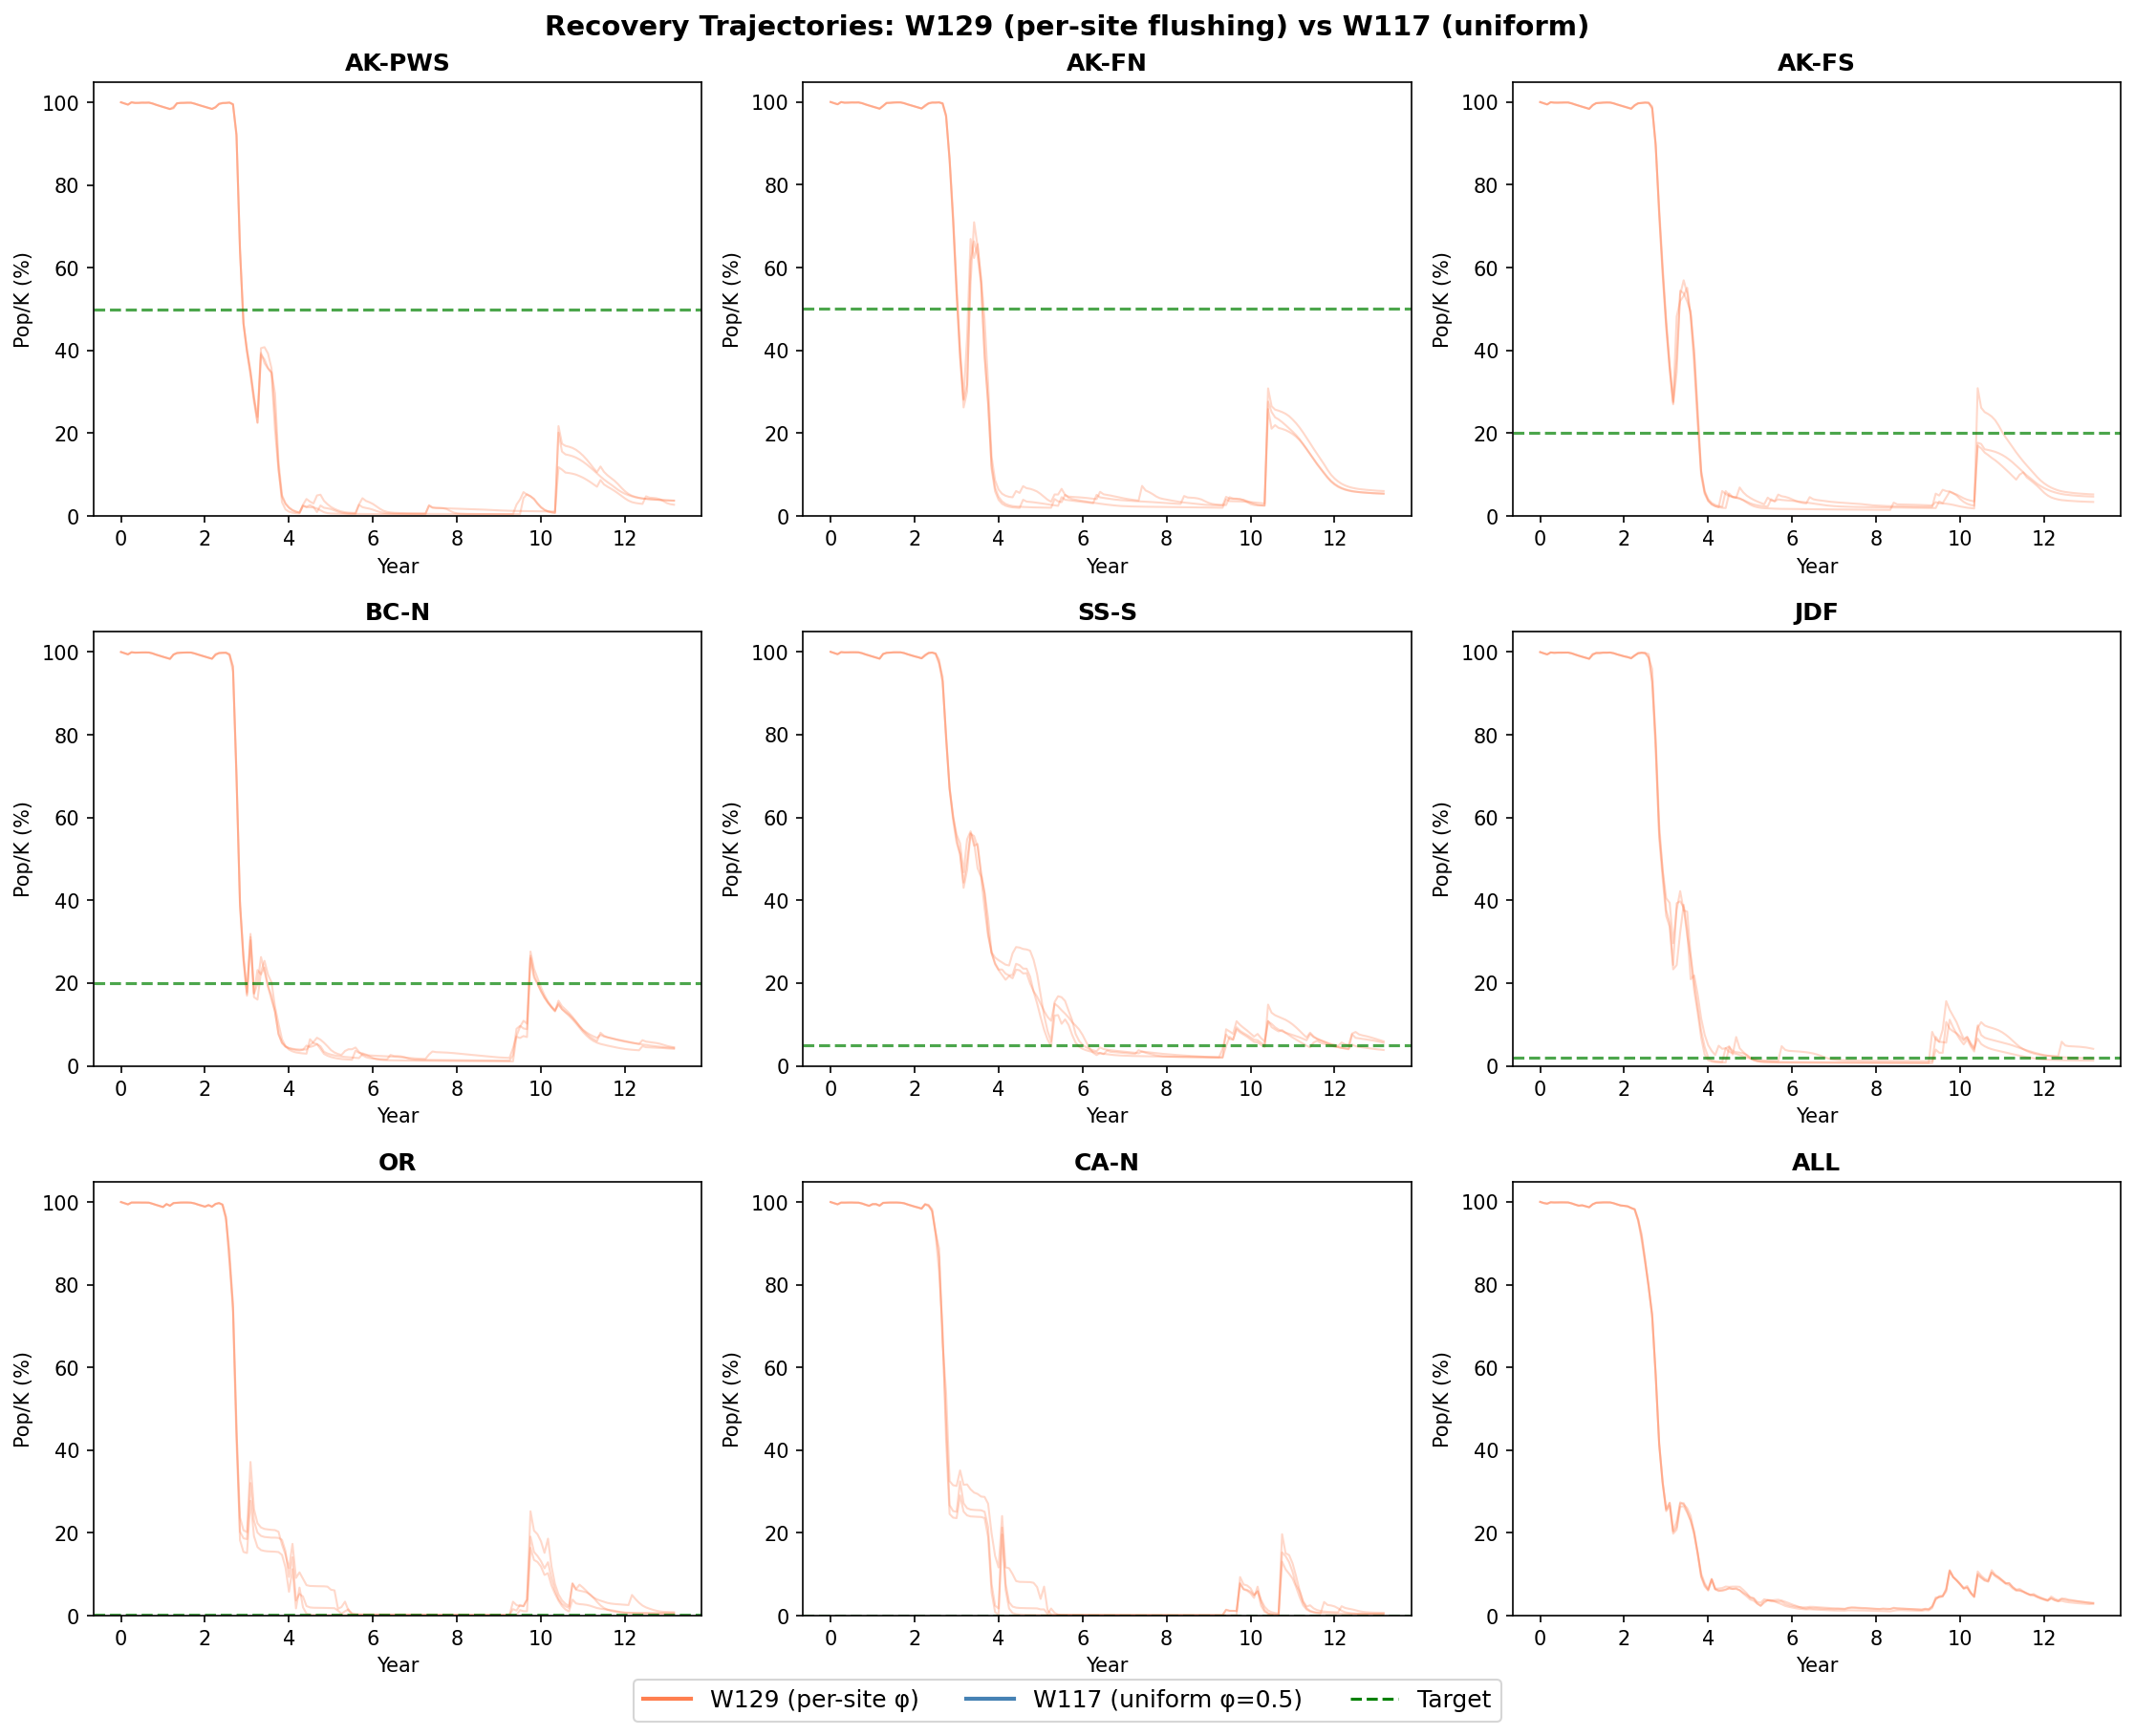
\includegraphics[width=\textwidth]{figures/fig4_trajectories.png}
\caption{Monthly recovery trajectories for all 8 scored regions plus overall. Orange = W129 (per-site $\phi$), blue = W117 (uniform). Dashed green = target. AK regions are worse under per-site flushing; southern regions show slightly more recovery.}
\end{figure}

\subsection{All Runs Heatmap}

\begin{figure}[h]
\centering
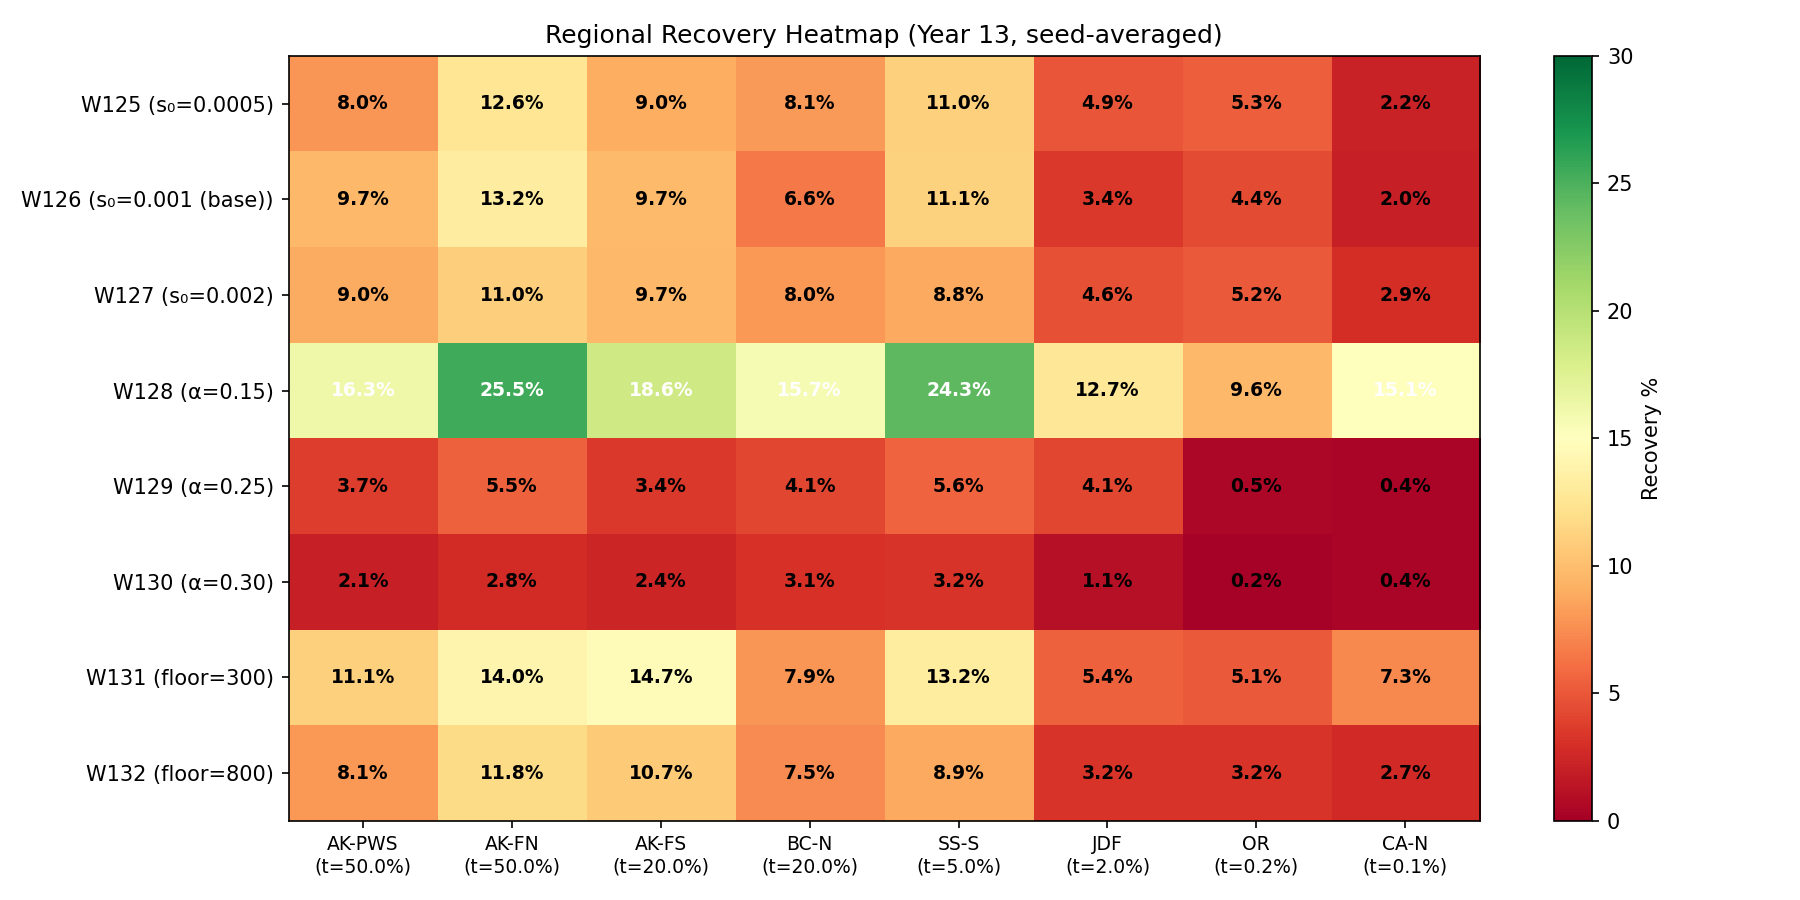
\includegraphics[width=\textwidth]{figures/fig5_heatmap.png}
\caption{Regional recovery heatmap across all 8 runs. Note W128 ($\alpha=0.15$, low disease amplification) has the highest AK recovery but also unacceptable southern recovery ($>$15\% in CA-N). The gradient-forming mechanisms conflict.}
\end{figure}

\subsection{Per-Region Error Diagnosis}

\begin{figure}[h]
\centering
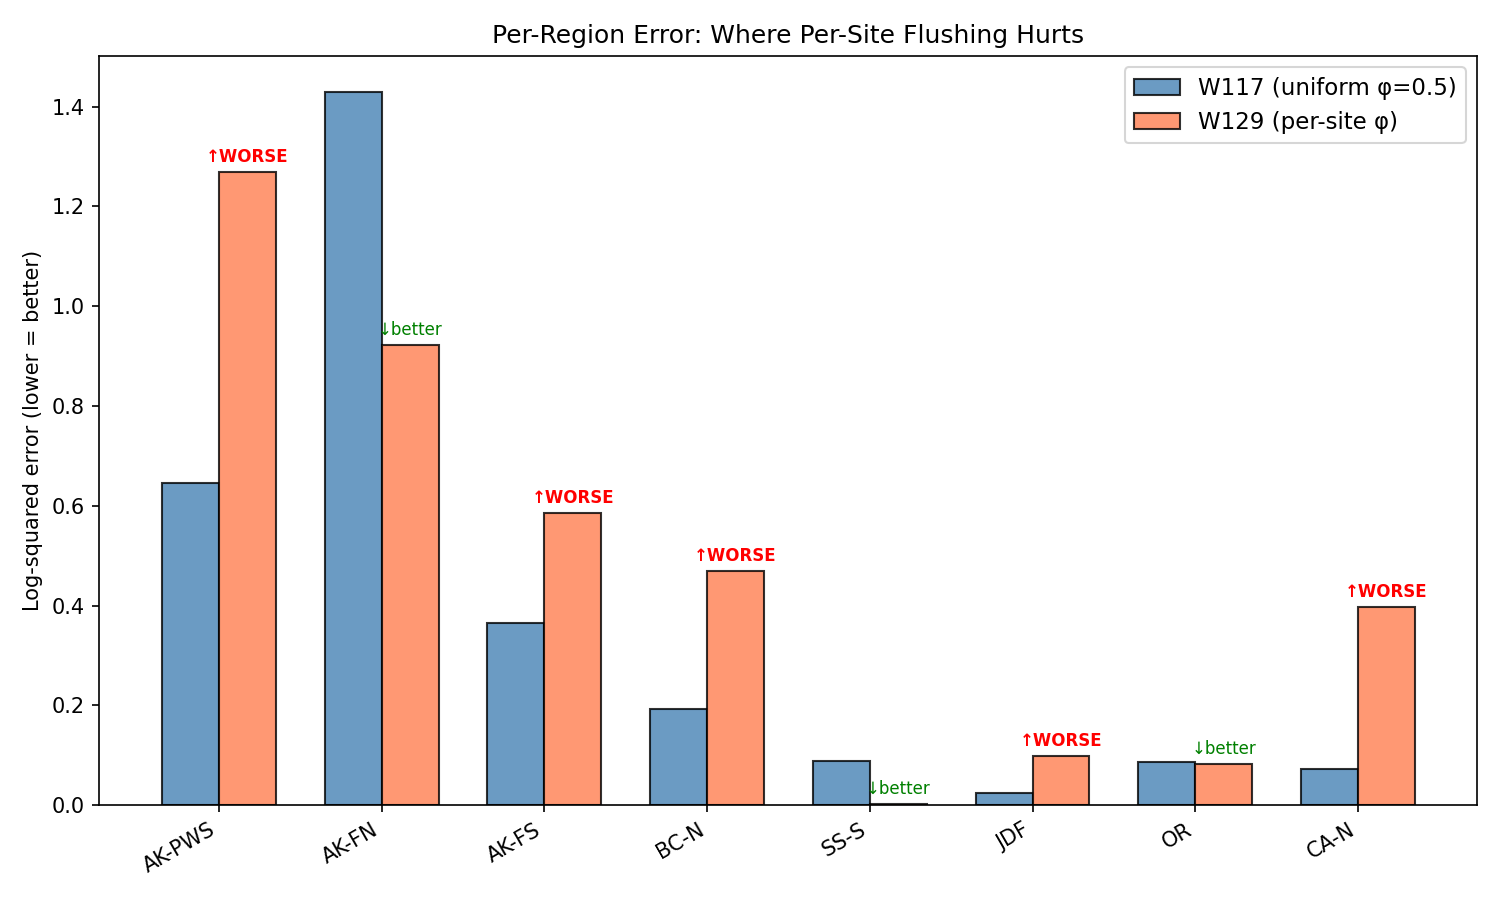
\includegraphics[width=\textwidth]{figures/fig6_diagnosis.png}
\caption{Where RMSE gets worse. W129 (orange) has higher error than W117 (blue) in AK-PWS, AK-FS, JDF, and CA-N. Only AK-FN and SS-S are comparable. The damage is spread across both ends of the gradient.}
\end{figure}

\subsection{Alpha Sensitivity}

\begin{figure}[h]
\centering
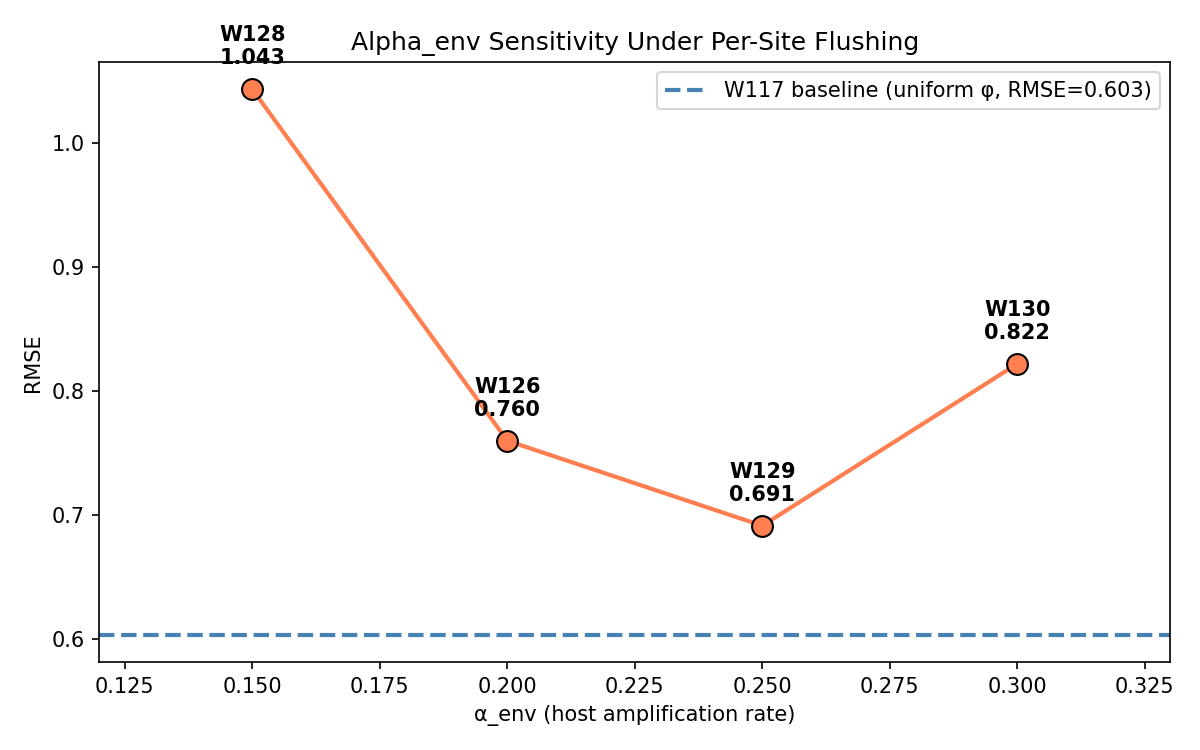
\includegraphics[width=\textwidth]{figures/fig7_alpha_sensitivity.png}
\caption{$\alpha_\text{env}$ sensitivity under per-site flushing. Optimal at 0.25 (W129), but no value reaches the W117 baseline. The U-shape suggests $\alpha$ trades off north vs south: too low lets south recover, too high suppresses everything.}
\end{figure}

\section{Implications}

\subsection{Per-Site Flushing is Physically Correct but Incomplete}

The enclosedness-derived $\phi$ values are defensible: enclosed waterways do retain water and pathogens longer. The problem is that our model lacks the \textbf{compensating mechanism} that makes enclosed waterways refuges in reality: \textit{salinity inhibition of Vibrio}.

\subsection{What n\_connectivity Might Do}

The W135--W144 round tests $n_\text{connectivity}$ = 0.5 and 2.0. With $n=0.5$, the $\phi$ values compress toward midrange (less extreme differentiation). This might soften the damage but won't fix the fundamental direction. With $n=2.0$, the contrast sharpens---likely worse.

\subsection{Possible Paths Forward}

\begin{enumerate}
    \item \textbf{Add salinity mechanism}: Per-node salinity modulation of \textit{Vibrio} activity. Freshwater-influenced sites get reduced $P_\text{env}$ amplification. This is the biologically correct fix (Gehman 2025).
    \item \textbf{Decouple import vs retention}: Let $\phi$ modulate the D matrix (import/export) but use a uniform rate for local $P_\text{env}$ decay. Enclosed sites would be protected from import without accumulating local pathogen.
    \item \textbf{Reverse the sign}: Use enclosedness to \textit{reduce} disease pressure rather than increase it (encode the net protective effect directly).
    \item \textbf{Revert to uniform $\phi$}: Accept that without salinity data, spatially-variable flushing hurts more than it helps.
\end{enumerate}

Option 1 is the most scientifically defensible. Option 2 is a quick mechanical fix. Option 4 is the pragmatic choice if we want to move to SA and paper writing.

\section{Summary Table}

\begin{table}[h]
\centering
\begin{tabular}{llrrrrrr}
\toprule
Run & Config & RMSE & AK-PWS & AK-FN & BC-N & SS-S & CA-N \\
\midrule
W117 & uniform $\phi$=0.5 & \textbf{0.603} & 7.85 & 3.19 & 7.27 & 2.52 & 0.19 \\
\midrule
W125 & s$_0$=0.0005 & 0.797 & 7.95 & 12.59 & 8.12 & 11.03 & 2.17 \\
W126 & s$_0$=0.001 & 0.760 & 9.66 & 13.25 & 6.61 & 11.14 & 2.03 \\
W127 & s$_0$=0.002 & 0.814 & 8.97 & 11.00 & 7.98 & 8.81 & 2.88 \\
W128 & $\alpha$=0.15 & 1.043 & 16.25 & 25.49 & 15.69 & 24.27 & 15.11 \\
W129 & $\alpha$=0.25 & 0.691 & 3.74 & 5.48 & 4.14 & 5.62 & 0.43 \\
W130 & $\alpha$=0.30 & 0.822 & 2.11 & 2.81 & 3.08 & 3.17 & 0.38 \\
W131 & floor=300 & 0.899 & 11.06 & 13.95 & 7.92 & 13.19 & 7.30 \\
W132 & floor=800 & 0.763 & 8.07 & 11.80 & 7.50 & 8.85 & 2.67 \\
\midrule
\multicolumn{2}{l}{Target} & --- & 50.0 & 50.0 & 20.0 & 5.0 & 0.1 \\
\bottomrule
\end{tabular}
\caption{Recovery percentages at year 13 (seed-averaged). All per-site flushing runs are worse than W117.}
\end{table}

\end{document}
